\documentclass[
    12pt,
    a4paper,
    oneside,
    bibliography=totoc,
    listof=totoc
]{scrbook}

\usepackage[utf8]{inputenc}
\usepackage[ngerman]{babel}
\usepackage[T1]{fontenc}

\usepackage{graphicx}
\usepackage{booktabs}

% Kopf- und Fußzeile
\usepackage[headsepline,footsepline]{scrlayer-scrpage}
\clearpairofpagestyles
\automark{chapter}
\ihead{Maximilian Stock -- 166816}
\ohead{\headmark}
\cfoot{\pagemark}
\pagestyle{scrheadings}
\renewcommand*{\chapterpagestyle}{scrheadings}


\usepackage[backend=bibtex, style=numeric]{biblatex}
\addbibresource{references.bib}

\usepackage[hidelinks]{hyperref}

\usepackage{parskip}

\usepackage[fleqn]{amsmath}

\graphicspath{{bilder/}}

\usepackage{subcaption}

\usepackage{wrapfig}

\usepackage{array}




\titlehead{{\Large Friedrich-Schiller-Universität Jena} \\
    Fakultät für Mathematik und Informatik \\
    \centering
    
\includegraphics[width=0.5\textwidth]{fsu_logo.jpg}}
\subject{\LaTeX\ Grundlagen}
\title{Elo-Zahl}
\subtitle{Ein Wikipediaartikel als Kreativprojekt}
\author{Maximilian Stock}
\date{\today}




\begin{document}

\frontmatter

\maketitle

\tableofcontents
\listoffigures
\listoftables


\mainmatter

%\chapter{Einleitung}

\clearpage
\markboth{}{}
\thispagestyle{plain} %Damit auf der Seite oben nicht "Tabellenverzeichnis" steht.

Die \textbf{Elo-Zahl} (auch \textbf{Elozahl}) ist eine Wertungszahl, welche die Spielstärke von Schachspielern (\autoref{fig:schach}) beschreibt. Sie wurde nach ihrem Erfinder Arpad Elo benannt. Inzwischen wurde das Konzept auch für andere Spiele (\autoref{fig:go}) und Sportarten adaptiert (s.\,u.).

Ausgehend vom \textit{Bradley-Terry-Modell} (benannt nach R. A. Bradley und M. E. Terry, die es im Jahr 1952 präsentierten), das wiederum auf einer Arbeit von Ernst Zermelo aus den 1920er Jahren basiert, entwickelte Arpad Elo 1960 ein objektives Wertungssystem für den US-amerikanischen Schachverband USCF. Es wurde 1970 auf dem Kongress in Siegen vom Weltschachverband FIDE übernommen. Der Weltschachverband nennt sein System \textit{FIDE rating system}. Eine Wertungszahl heißt offiziell \textit{FIDE rating}, wird umgangssprachlich aber zumeist einfach als \glqq Elo-Zahl\grqq\ bezeichnet. Neben dem internationalen Wertungssystem der FIDE existieren auch nationale Wertungssysteme mit unterschiedlichen Namen. In Deutschland heißt das nationale Wertungssystem \textit{Deutsche Wertungszahl (DWZ)}, in Österreich werden \textit{(nationale) Elo-Zahlen} berechnet, und in der Schweiz gibt es eine \textit{Führungsliste} mit \textit{Führungszahlen}. Diese Systeme werten wesentlich mehr lokale Turniere aus, berechnen die Wertungszahlen aber ebenso nach den Methoden von Arpad Elo mit meist nur geringen Modifikationen und abweichenden Faktoren.

\begin{figure}[htbp]
    \centering
    \begin{subfigure}[b]{0.48\textwidth}
        \centering
        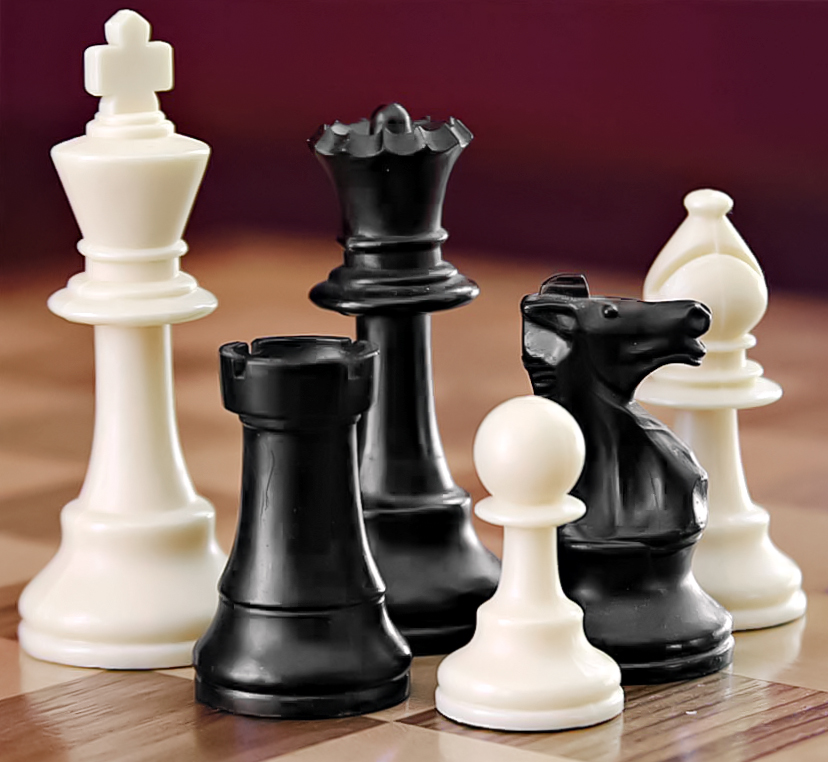
\includegraphics[width=\textwidth]{schach.jpg}
        \caption{Schach}
        \label{fig:schach}
    \end{subfigure}
    \hfill
    \begin{subfigure}[b]{0.48\textwidth}
        \centering
        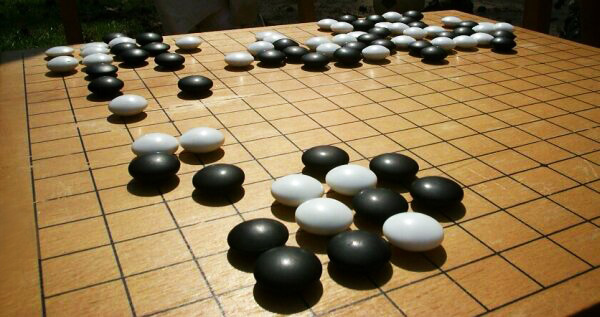
\includegraphics[width=\textwidth]{go.jpg}
        \caption{Go}
        \label{fig:go}
    \end{subfigure}
    \caption{Sowohl bei Schach- also auch bei Go-SpielerInnen kann die Elo-Zahl die Spielstärke beschreiben.}
    \label{fig:schach_go}
\end{figure}
\chapter{Grundprinzip}

Jedem Spieler ist eine Elo-Zahl $R$ (von englisch \textit{rating}) zugeordnet. Je stärker der Spieler, desto höher die Zahl. Treten mehrere Spieler gegeneinander an, so lässt sich aus den Elo-Zahlen der Spieler die erwartete Punktezahl der jeweiligen Spieler bestimmen.

Nach der Begegnung wird das Elo-Rating der Spieler ihren Ergebnissen angepasst. Je nach Differenz zwischen Erwartungswert und Ergebnis gewinnt ein Spieler Elo-Rating-Punkte hinzu oder verliert sie. Das System ist so konstruiert, dass Elo-Rating-Punkte im Regelfall (s. Anm. \ref{anm_1}) unter den beteiligten Spielern umverteilt werden.
\chapter{Berechnung}

\section{Erwartungswert}

Bei einer Begegnung zweier Spieler gibt es für einen Sieg einen, für ein Unentschieden einen halben und für eine Niederlage keinen Punkt. Die \textit{erwartete Punktezahl E} (von englisch \textit{expected score}, Erwartungswert) ist somit die Wahrscheinlichkeit, dass der Spieler gewinnt, multipliziert mit einem Punkt, plus die Wahrscheinlichkeit für ein Remis multipliziert mit einem halben Punkt. Der Erwartungswert liegt damit zwischen $0$ und $1$. %TODO: Verweis auf Anmerkung 2 :)

Das Elo-System ist mathematisch so modelliert, dass sich bei der Begegnung zweier Spieler $A$ und $B$ der Erwartungswert $E_{A}$ für den Spieler $A$ aus den beiden Ratings $R_{A}$ und $R_{B}$ wie folgt berechnet:

%PLATZHALTER: Formel für E_A

Entsprechend gilt für $E_{B}$, den erwarteten Punktestand von Spieler $B$:

%PLATZHALTER: Formel für E_B (einfach kopieren von oben).

Da genau ein Punkt auf beide Spieler verteilt wird, muss gelten:

%PLATZHALTER: Formel EA und EB einfügen.

%PLATZHALTEN: Tabelle mit Werten für E_A und E_B eventuell (daneben??) einfügen

Aus den Formeln für den Erwartungswert ergibt sich, dass diese Bedingung stets erfüllt ist.

Die in der Formel enthaltene, willkürlich festgelegte Zahl $400$ legt die Abstufung der Elo-Skala fest: Bei einer Elo-Differenz von $400$ wird der Spieler höchstwahrscheinlich gewinnen ($E_{A} = 91 \%$). Die Zahl $400$ wurde von Arpad Elo so gewählt, damit die Elo-Zahlen mit den Wertungszahlen des früher verwendeten Schach-Rating-Systems von Kenneth Harkness möglichst gut kompatibel sind. Im Schweizer Tischtennis wird z.\,B. $200$ statt $400$ verwendet, im deutschen $150$, s.\,u. %TODO: mögliche Anmkerung 3

Beträgt der Wertungsunterschied $|R_{B} - R_{A}|$ mehr als $400$ Punkte, so erlaubt die FIDE anstelle der tatsächlichen Differenz den Wert $400$ bzw. $-400$ zu benutzen. Ab 2022 kann ein Spieler aber nur noch einmal pro Turnier von einer solchen Aufwertung profitieren, für die anderen eventuellen Gegner mit einem Wertungsunterschied $> 400$ wird dann mit dem tatsächlichen Wertungsunterschied gerechnet.

%Hier ist auf Wikipedia angemerkt, dass kommende Abschnitte überarbeitet werden müssen.

Die Gewinnerwartung eines Spielers als Funktion der Punktedifferenz folgt in Elos Modell einer logistischen Funktion. Das heißt jedoch \textit{nicht}, dass die Stärken der Spieler logistisch verteilt sind. Elo verzichtet auf eine solche Verteilungsannahme. Sein Modell fußt auf der charakteristischen Eigenschaft der \textit{Multiplikativität der Erwartungswerte}.


\section{Multiplikativität der Erwartungswerte}

Die Erwartungswerte sind multiplikativ -- mithilfe dieser Eigenschaft lässt sich Elos Modell definieren. Wenn etwa Spieler $A$ gegenüber Spieler $B$ ein $3$:$1$-Favorit ist (d.\,h., $A$ erzielt in Partien gegen $B$ $75$ Prozent der Punkte) und $B$ gegenüber $C$ ein $2$:$1$-Favorit, so fordert bzw. folgt aus Elos Modell, dass $A$ gegenüber $C$ ein $6$:$1$-Favorit ist.

Oder allgemein ausgedrückt:

%PLATZHALTER: Alignment mit den drei Aussagen einbauen (oder so)

Dies kann man leicht nachrechnen. Die \textit{Multiplikativität} ist aber \textit{keine} Konsequenz aus einer Normalverteilung, was man oft liest. Diese bezieht sich nur auf die Abweichung der tatsächlichen Spielergebnisse eines Spielers vom Erwartungswert (s.\,u.) und nicht auf eine Normalverteilung der Stärken der Spieler. Die Forderung nach Multiplikativität stellt den besseren Ausgangspunkt für die Entwicklung des Modells dar -- insbesondere für die Kalkulation der Spielstärken von Spielern früherer Epochen.


\section{Anpassung der Elo-Zahl}

Die Elo-Zahlen der Spieler werden regelmäßig aktualisiert. Erzielt ein Spieler in seinen Partien mehr Punkte, als von seiner aktuellen Elo-Zahl zu erwarten war, gewinnt er Elo-Punkte hinzu; erzielt er weniger, verliert er Elo-Punkte. Maßgeblich ist hierfür der so genannte $k$-Faktor oder $k$-Koeffizient. Er gibt an, wie viele Elo-Punkte ein Spieler bei einer Partie maximal hinzugewinnen kann (bei einem Sieg über einen viel stärker bewerteten Gegner) oder maximal verlieren kann (Niederlage gegen einen viel schwächer bewerteten Gegner). Wenn ein Spieler $S$ Partiepunkte erzielt, der Erwartungswert aufgrund bestehender Elo-Zahlen aber $E$ betrug, ändert sich seine Elo-Zahl um $k \cdot (S - E)$. Die neue Elo-Zahl $R'$ ist also

%PLATZHALTER: Formel für R' einfügen

Der Faktor $k$ ist durch das Elo-Modell nicht festgelegt. Wenn er sehr groß gewählt wird, wirken sich zufällige Einzelergebnisse stark aus: die Elo-Zahl $R$ kann stark schwanken. Wenn er sehr klein gewählt wird, ist die Anpassung \glqq träge\grqq : $R$ wird erst nach vielen Partien an eine reale Änderung der Spielstärke angepasst. Für Spitzenspieler mit eher konstanter Leistung ist ein kleinerer Faktor angebracht als für Anfänger, die schnell Fortschritte machen können. Der Koeffizient $k$ wird daher dem \glqq Entwicklungsstand\grqq\ eines Spielers angepasst.%TODO: Anmkerung 1 verweisen

Im Schach hat $k$ im Regelfall den Wert $40$, $20$ oder $10$:
\begin{itemize}
    \item $k = 40$: für Spieler, die neu in der Ratingliste sind und weniger als dreißig gewertete Partien aufweisen;
    \item $k = 40$: für alle Spieler bis zum Ende des Kalenderjahres ihres 18. Geburtstags, solange ihre Bewertung $< 2300$ bleibt;
    \item $k = 20$: für alle Spieler mit mindestens dreißig gewerteten Partien und einer maximalen Elo-Zahl $< 2400$. Dieser $k$-Wert trifft für die meisten erwachsenen Spieler zu;
    \item $k = 10$: für alle Top-Spieler, die eine Elo-Zahl $\geq 2400$ erreicht haben, selbst wenn die Elo-Zahl wieder unter diesen Wert fällt.
\end{itemize}

Ausnahmsweise kann $k$ für einen Spieler in einer einzelnen Wertungsperiode einen abweichenden Wert annehmen, da das Produkt aus $k$ und der Anzahl der für einen Spieler in einer Wertungsperiode ausgewerteten Partien ($n$) kleiner als $700$ sein muss. In diesem Fall wird $k$ auf die größte natürliche Zahl abgesenkt, für die $k \cdot n < 700$ gilt.





\subsection{Anpassung nach einer Partie}

\subsection{Maximaler Punktgewinn durch eine Partie}

\subsection{Spiele gegen einen gleichstarken Spieler}




\section{Elo-Performance}




\chapter{Probleme und statistische Phänomene von Rating-Systemen}

\section{Intransitivität von Wahrscheinlichkeitsrelationen}

Ist Spieler $A$ gegenüber Spieler $B$ der Favorit und $B$ gegenüber $C$, so besitzt $A$ ein höheres Rating als $B$ und $B$ ein höheres als $C$. Damit besitzt $A$ ein höheres Rating als $C$ und \textit{müsste} Favorit gegenüber $C$ sein.

Diese Folgerung ist aber keineswegs zwingend, da Wahrscheinlichkeits- bzw. Präferenzrelationen nicht notwendigerweise transitiv sind. Dieses Problem ist keine Besonderheit des Elo-Systems, sondern ein prinzipielles Problem aller Rating-Systeme. (vgl. Condorcet-Paradoxon, \glqq Chinesische Würfel\grqq\ oder \glqq Intransitive Würfel\grqq )

Transitivität ist jedoch eine notwendige Voraussetzung für ein sinnvolles Rating-System. Um diese Eigenschaft zu sichern, setzte Arpad Elo bei der Entwicklung seines Rating-Systems voraus, dass das zu erwartende Spielergebnis in Abhängigkeit der Spielstärken mithilfe der Formel $E_{A} = 1 / (1 + 10^{(R_{B} - R_{A}) / 400})$ beschreibbar ist. Aus dieser Annahme folgt neben der Transitivität auch die oben dargestellte Multiplikativität der Erwartungswerte.


\section{Deflation und Inflation}

Will man mithilfe der Elo-Zahlen -- oder anderer Ratings, dies betrifft nicht nur das Elo-System -- die Stärken von Spielern aus unterschiedlichen Epochen vergleichen, so sollte ein Rating von z.\,B. $1600$ aus dem Jahre 1970 gleichbedeutend mit einem Rating von $1600$ aus dem Jahre 2000 sein. Insbesondere sollte, da sich infolge der Weiterentwicklung der Theorie die durchschnittliche Spielstärke im Laufe der Zeit zumindest nicht verschlechtert, sich die mittlere Ratingzahl nicht verringern.

Beim Elo-System gewinnt der Sieger einer Partie genau so viele Rating-Punkte hinzu, wie der Verlierer einbüßt (falls beide den gleichen $k$-Faktor zur Berechnung nutzen): die mittlere Spielstärke beider bleibt gleich. Umfasst der \textit{Rating-Pool} (die Rangliste) nur starke Spieler, so ist folgendes Phänomen zu beobachten: Sooft ein Spieler neu in die Ratings aufgenommen wird, tritt er mit einer gewissen (niedrigen) Punktezahl ein. Im Laufe seiner Karriere verbessert er seine Stärke, gewinnt Punkte hinzu und scheidet später mit einer (hohen) Punktezahl aus -- dadurch werden der Gesamtheit Punkte entzogen, und die mittlere Ratingzahl sinkt; d.\,h., das System ist deflationär.

Vergrößert man den Rating-Pool auch auf schwächere Spieler, so tritt der entgegengesetzte Effekt auf: Viele Spieler verlassen den Rating-Pool mit einem niedrigeren Rating, als ihnen bei Eintritt zugemessen wurde -- das System wird nun inflationär.

Dies war insbesondere früher der Fall, als der Weltschachbund FIDE Schachspieler erst ab einer Wertungszahl von $2200$ in die Rangliste aufnahm. Da die Elo-Auswertung von Turnieren gebührenpflichtig ist und damit für die FIDE eine Einnahmequelle darstellt, wurde diese Schwelle immer weiter herab gesenkt, zuletzt auf $1000$. Dennoch lässt es sich nicht vermeiden, dass viele Spieler den Rating-Pool mit niedrigeren Wertungszahlen verlassen als sie bei Eintritt erhielten. Eine maßvolle Inflation ist jedoch durchaus erwünscht, diese sollte in ihrem Ausmaß der Weiterentwicklung der Spielstärken im Laufe der Zeit Rechnung tragen, allerdings ergibt sich hier zumeist das Problem einer zu großen Inflation.

So konnten die Elo-Zahlen immer neue Rekorde erreichen, ohne eigentlich noch ein absolutes Maß für die Spielstärke zu sein. Im Jahr 2000 gab es nur einen Spieler (Kasparow) mit einer Elo-Zahl größer $2800$, elf Spieler größer $2700$, und etwa $90$ erreichten einen Wert über $2600$. Im Juli 2010 hatten bereits über $200$ aktive Spieler eine Elo-Zahl größer $2600$, davon $37$ mindestens $2700$; drei Spieler hatten sogar eine Elozahl von $2800$ oder höher, was 20 Jahre zuvor undenkbar schien.

Die durchschnittliche Elo-Zahl der ersten $100$ Spieler der Weltrangliste stieg zwischen Juli 2000 und Juli 2012 von $2644$ auf $2703$ Punkte, also eine Steigerung um $59$ Wertungspunkte. Von 2012 bis 2023 lag der Mittelwert recht konstant zwischen $2700$ und $2706$, seit 2024 liegt er unter $2700$.


\section{Das Tausend-Partien-Problem}

Ein weiteres Phänomen ist das sogenannte \textit{Tausend-Partien-Problem}. Oft treffen Spieler der gleichen Spielstärke immer wieder aufeinander. Angenommen, zwei Spieler mit Elo $2000$ spielen zehn Partien, bei denen der eine $80 \%$ der Punkte erreicht. Nach der Berechnung der neuen Elo-Zahl ergeben sich die Werte $2080$ für den Sieger und $1920$ für den Verlierer. Tragen die beiden Spieler jedoch $1000$ Partien mit gleichem Punkteverhältnis aus, ohne dass die Wertung aktualisiert wird, so ergibt sich für den Sieger eine neue Wertungszahl, die höher als die des aktuellen Weltmeisters ist. Jedoch ist dieses Szenario nur theoretischer Natur. Nach dem Statistikgesetz der großen Zahl darf man erwarten, dass die beiden gleich starken Spieler (beide hatten Elo $2000$) sich nach vielen Partien den zu erwartenden $50 \%$ annähern. Zudem wird es in der Praxis nie $1000$ Partien ohne Ratingaktualisierung geben.

Die Entwicklung der Wertzahlen wird auch von der Auswertungsperiode beeinflusst. Nach einer Testphase mit unregelmäßigen Veröffentlichungen wurde von 1975 bis 1980 einmal jährlich im Januar eine neue Liste veröffentlicht. Beginnend im Juli 1981 wurde auf halbjährliche Veröffentlichung umgestellt und dies bis Juli 2000 so beibehalten. Im Oktober 2000 wurde dann auf Veröffentlichung alle drei Monate umgestellt. Von Juli 2009 bis Juli 2012 wurde alle zwei Monate ausgewertet. Seit August 2012 wird monatlich ausgewertet. Die minimale Wertungszahl beträgt seitdem 1000 Punkte, zuvor lag sie bei 1200. Sinnvoll wäre prinzipiell eine Auswertung nach jedem Turnier, da so Formschwankungen von Spielern besser ausgeglichen werden können. Allerdings ist das derzeit nicht geplant.


\section{Schwankungsbreite und Aussagekraft}

Die Wertungszahlen eines einzelnen Spielers sind intervallskaliert und annähernd normalverteilt und schwanken mit einer Standardabweichung von $200$ um einen mittleren Wert. Es gibt viele Schachspieler mit Spielstärken unter $1200$. Auf diesem Spielniveau ist das Elo-System in der Vorhersagesicherheit aber nur eingeschränkt anwendbar. Wichtig ist insbesondere auf Hobbyspielerniveau, dass ein Spieler seine Zahl auch gegen stärkere Gegner verteidigen kann, ohne sich auf besondere Eigenschaften wie unbewusste psychische Schwächen oder schlechtes Zeitmanagement von Neulingen konzentrieren zu müssen. Utopisch hohe Werte werden durch Niederlagen schnell, exakt und zuverlässig korrigiert. Die recht stabile Elo-Zahl wird mit verschiedenen Verfahren ermittelt. Manche gehen von wenigen Spielen aus oder von ähnlich starken Turnierteilnehmern. Nach vielen Partien erreichen aber alle sehr ähnliche Gleichgewichte. Bei Computern ist die Verteilung nicht nur per $200$-Punkte-Definition gleich, sondern auch vom Kurvenverhalten her darüber hinaus sehr ähnlich, allerdings gibt es bei ähnlich starken Maschinen eine weitere Spielstärkenspreizung in den verschiedenen Partiephasen.
\chapter{Schach}

\section{Einstufung der Spieler nach Elo-Zahl}

Vor Einführung der Elo-Zahl stufte man die Spieler beim Schach in neun Klassen oder Kategorien ein. Ein Unterschied von einer Klasse bedeutete, dass der bessere Spieler als Ergebnis einer Partie $0,75$ Punkte \textit{erwarten} darf. Im Elo-System entspricht dieser Spielstärkeunterschied einer Differenz von etwa $200$ Wertungspunkten (genauer: $191$, s. Anm. \ref{anm_5}). Eine Erweiterung stellt das Glicko-System dar.

\begin{table}[htbp]
    \centering
    \begin{tabular}{c >{\centering\arraybackslash}p{6.2cm} >{\centering\arraybackslash}p{6.2cm}}
        \toprule
        \textbf{Elo-Zahl} & \textbf{Offene Kategorie} & \textbf{Kategorie Frauen} \\
        \midrule
        $\geq 2500$     & \multicolumn{2}{c}{Großmeister (GM)} \\
        $2400 - 2499$  & \multicolumn{2}{c}{Internationaler Meister (IM)} \\
        $2300 - 2399$  & FIDE-Meister (FM) & Großmeister der Frauen (WGM) \\
        $2200 - 2299$  & Candidate Master (CM) oder Nationaler Meister & Internationaler Meister der Frauen (WIM) \\
        $2100 - 2199$  & Meisteranwärter & FIDE-Meister der Frauen (WFM) \\
        $2000 - 2099$  & Starker Amateur & Candidate Master der Frauen (WCM) \\
        $< 2000$        &  \multicolumn{2}{c}{Amateur} \\
        \bottomrule
    \end{tabular}
    \caption{Zuordnung der Titel nach der Wertungszahl.}
    \label{tab:schach-titel}
\end{table}

Zu beachten ist dabei, dass man die verschiedenen Titel Großmeister (GM) und Internationaler Meister (IM) nicht nur auf Grund einer bestimmten Elo-Zahl erhält, sondern durch die Erfüllung von anderen festgelegten Normen. Um den Titel nach Erfüllung aller Normen zu erhalten, muss ein angehender GM allerdings eine Elo-Zahl von mindestens $2500$, ein IM eine Zahl von mindestens $2400$ einmal erreicht haben. Bei entsprechender Punktzahl wird der offene Großmeistertitel an Spieler aller Geschlechter vergeben, der Großmeistertitel der Frauen kann von diesen bereits ca. $200$ Punkte vorher erreicht werden (\autoref{tab:schach-titel}).

Unterhalb $2000$ Elo-Punkten gibt es keine offiziellen Titel, weshalb eine objektive Benennung der Spielstärke schwierig ist. Zur groben Einschätzung kann in Deutschland der DWZ-Schnitt der Amateurligen dienen (Die Deutsche Wertzahl DWZ ist zwar nicht dasselbe wie die international übliche Elo-Zahl, aber vergleichbar). Im Schachverband Württemberg liegt der DWZ-Schnitt in der Oberliga bei ca. $2100$, in den Verbandsligen bei ca. $1900$, in den Landesligen bei ca. $1700$, den Bezirksligen bei ca. $1600$ usw. Wie in anderen Sportarten auch erreichen Gelegenheitsspieler selten das Niveau der Bezirksliga.

\begin{wraptable}{r}{0.37\textwidth}
    \centering
    \begin{tabular}{c c c}
        \toprule
        \textbf{Turnier-} & \multicolumn{2}{c}{\textbf{Elo-Durchschnitt}} \\
        \textbf{kategorie} & \textbf{Von} & \textbf{Bis} \\
        \midrule
        \textbf{1} & $2251$ & $2275$ \\
        \textbf{2} & $2276$ & $2300$ \\
        \textbf{3} & $2301$ & $2325$ \\
        \multicolumn{3}{c}{$\dots$} \\
        \textbf{7} & $2401$ & $2425$ \\
        \multicolumn{3}{c}{$\dots$} \\
        \textbf{11} & $2501$ & $2525$ \\
        \multicolumn{3}{c}{$\dots$} \\
        \textbf{15} & $2601$ & $2625$ \\
        \multicolumn{3}{c}{$\dots$} \\
        \textbf{19} & $2701$ & $2725$ \\
        \textbf{20} & $2726$ & $2750$ \\
        \textbf{21} & $2751$ & $2775$ \\
        \textbf{22} & $2776$ & $2800$ \\
        \textbf{23} & $2801$ & $2825$ \\
        \bottomrule
    \end{tabular}
    \caption{Turnier-Kategorien.}
    \label{tab:turnier-kategorien}
\end{wraptable}

Nachdem im Jahr 1970 die Elo-Zahl als Wertungssystem eingeführt worden war, hatte zunächst Bobby Fischers Bestmarke von $2785$ Punkten vom Juli 1972 für viele Jahre Bestand. Im Jahre 1999 erreichte der damalige klassische Schachweltmeister Garri Kasparow die Elo-Zahl von $2851$ Punkten, die erst im Januar 2013 von Magnus Carlsen mit $2861$ Punkten übertroffen wurde. Inzwischen konnte Carlsen den Rekord auf $2882$ erhöhen (Mai 2014 und August 2019).

Spieler mit einer Elo-Zahl über $2600$ gehören zum erweiterten Kreis der Weltspitze (etwa TOP $200$), Spieler mit über $2700$ zum engeren Kreis (etwa TOP $30$). Aktuell (Stand: Dezember 2025) erreichen nur zwei Spieler $2800$, und zwar Hikaru Nakamura sowie Magnus Carlsen.

Elo-Zahlen können auch für einzelne Turniere berechnet werden (s.\,o.: \textit{Elo-Performance}). Hierbei gelang Fabiano Caruana im Jahr 2014 beim Turnier um den Sinquefield Cup in St. Louis eine Elo-Leistung von $3103$. Die davor gültige höchste Turnier-Elo-Leistung war $3002$, erzielt von Magnus Carlsen in Nanjing im Jahr 2010. \cite{loeffler2014}


\section{Historische Elo-Zahl im Schach}

Für den Vergleich heutiger Spitzenspieler mit Großmeistern vor der Einführung der Elo-Zahl wird die sogenannte historische Elo-Zahl verwendet. %TODO: ggf Hauptartikel verlinken

\section{Spielstärke der Schachprogramme}

Die Elo-Zahlen der Schachcomputer bzw. Computerprogramme sind nicht ohne weiteres mit denen menschlicher Schachspieler zu vergleichen, da sie überwiegend durch Partien zwischen Computern ermittelt wurden und nicht durch Teilnahme an offiziellen Turnieren. %TODO: ggf Hauptartikel verlinken


\section{Turnierkategorien -- Einteilung der Turniere nach Elo-Zahl}

Auch Rundenturniere werden nach der durchschnittlichen Elo-Zahl der Teilnehmer in Kategorien eingeteilt. Hierbei entspricht ein Unterschied um eine Kategorie $25$ Elo-Punkten (\autoref{tab:turnier-kategorien}). Als Turnier der Kategorie 1 wird dabei ein Turnier eingestuft, dessen Teilnehmer im Durchschnitt $2251$ bis $2275$ Elo-Punkte haben. Die zurzeit stärksten Turniere erreichen die Kategorie 22, was einem Durchschnitt von $2776$ bis $2800$ Elo-Punkten entspricht. Bei der Zürich Chess Challenge 2014 wurde im Januar 2014 erstmals Kategorie 23 (mit einem Elo-Durchschnitt von $2801$) erreicht.
\chapter{Weitere Anwendung und Verbreitung}

\section{Go}

Bei Go wird die Spielstärke traditionell in Kyū-Graden für Schüler und Dan-Graden für Meister angegeben. Die Ermittlung dieser Spielstärke basiert innerhalb der \textit{European Go Federation} und bei vielen Go-Servern im Internet auf einem von Elo abgeleiteten System, welches Kyū- und Dan-Grade wie folgt abbildet:

\begin{table}[htbp]
    \centering
    \begin{tabular}{l | c | l}
        \toprule
        \textbf{kyū/dan} & \textbf{Elo} & \textbf{Spielstärke und -erfahrung} \\
        \midrule
        weltbeste & $5185$ & AlphaGo Zero auf einem TPU-v2-Modul mit \\
        9p-KI & & 180 TFLOPS \cite{silver2017} \\
        weltbester & $3830$ & Shin Jin-Seo, weltbester Go-Spieler \\
        9p-Spieler & & \\
        1p - 9p & ab circa $2600$ & professioneller Go-Spieler (aus Japan, Korea oder \\
        & & China), der stärker als ein Amateur-6dan spielt \\
        4d - 7d & ab $2350$ & einer der besten Spieler seines Landes \\
        1d - 3d & $2050 - 2349$ & sehr guter Club-Spieler \\
        4k - 1k & $1650 - 2049$ & guter Club-Spieler \\
        9k - 5k & $1150 - 1649$ & regelmäßiger Club-Spieler \\
        13k - 10k & $750 - 1149$ & Club-Spieler \\
        17k - 14k & $350 - 749$ & regelmäßiger Hobby-Spieler \\
        21k - 18k & $0 - 349$ & Hobby-Spieler \\
        24k - 22k &  & einige Partien gegen Nicht-Anfänger gewonnen \\
        27k - 25k &  & einige Partien gegen Anfänger gewonnen \\
        29k - 28k &  & einige Partien gespielt \\
        30k &  & Regeln verstanden, aber noch keine Partie gespielt \\
        \bottomrule
    \end{tabular}
    \caption{Die European Go Federation leitet die Spielstärke aus der Elo ab.}
    \label{tab:go_elo}
\end{table}




\section{Fußball}

Die FIFA-Weltrangliste der Frauen wird seit 2003 offiziell mit einem adaptierten Elo-System ermittelt. Seit 2018 wird die FIFA-Weltrangliste für Männer auch auf ein adaptiertes Elo-System umgestellt. \cite{fifa2018weltrangliste}

Eine länger bestehende inoffizielle Adaption des Elo-Systems für Männernationalmannschaften im Fußball sind die World Football Elo Ratings. Inoffizielle Elo-Ratings werden auch für Fußball-Clubs vorgenommen.


\section{Tischtennis}

\subsection{In der Schweiz}

Swiss Table Tennis nutzt seit der Saison 2010/2011 eine etwas modifizierte Elo-Formel zur Berechnung von Wertungspunkten
\[
    E_{A} = \frac{1}{1 + 10^{(R_{B} - R_{A}) / 200}}
\]
\begin{itemize}
    \item[] $E_{A}$: Erwarteter Punktestand für Spieler $A$.
    \item[] $R_{A}$: bisherige Punkte-Zahl von Spieler $A$.
    \item[] $R_{B}$: bisherige Punkte-Zahl von Spieler $B$.
\end{itemize}
Der Erwartungswert von $A$ beträgt nun $E_{A} \cdot 100 \%$. Die neue Punkte-Zahl von Spieler $A$ ist
\[
    R'_{A} = R_{A} + 15 \cdot (S_{A} - S_{E})
\]
\begin{itemize}
    \item[] $S_{A}$: tatsächlich gespielter Punktestand ($1$ für jeden Sieg, $0$ für jede Niederlage, Remis ist im Tischtennis nicht möglich).
\end{itemize}


\subsection{In Deutschland: der TTR-Wert}

In Deutschland wird nach einem analogen System für jeden Aktiven ein \textbf{TTR-Wert} errechnet \cite{tischtennis2020heft11}. Hier wird die Wertungsdifferenz durch $150$ geteilt.
\[
    E_{A} = \frac{1}{1 + 10^{(R_{B} - R_{A}) / 150}}
\]


\section{Scrabble}

Für weltweites Scrabble (Global Scrabble) wird eine Elo-Rangliste von der World English-language Scrabble Players' Association (WESPA) geführt. Auf Rang 1 dieser Elo-Rang-liste liegt der Neuseeländer Nigel Richards ($2156$ Elo-Punkte, Stand 17. Oktober 2020).

Seit 2009 wird auch für das deutschsprachige Scrabble eine Elo-Rangliste geführt -- basierend auf Turnieren ab dem Jahr 2005. Im Juni 2022 führte der Deutsche Timon Boerner mit $1718$ Elo-Punkten die Liste an, in der $213$ Personen aufgeführt sind.


\section{League of Legends}

Im MOBA League of Legends, einer Liga eines Computer-Strategiespiels, wurde ebenfalls das Elo-System bei gewerteten Spielen verwendet. Inzwischen wurde es durch das Ligasystem ersetzt, dem aber noch das Elo-System zu Grunde liegt.

Bei einem Sieg bekommt man \textit{League Points} (LP), bei einer Niederlage werden LP abgezogen. Bis Ende 2020 musste man bei $100$ LP ein Best of three bzw. five gewinnen, um eine Liga aufzusteigen.


\section{Tennis-Elo-Wertungssystem}

Das Tennis-Elo-Wertungssystem berechnet das relative Leistungsniveau von Tennisspielern im Herreneinzel. Nach jedem Spiel erhält der Gewinner Punkte vom Verlierer. Die Anzahl der Punkte hängt von den relativen Wertungen der Spieler ab -- ein Sieg über einen Spieler mit höherer Wertung führt zu einer größeren Wertungssteigerung als ein Sieg über einen Spieler mit niedrigerer Wertung. Die Wertungen liegen bei Profispielern typischerweise zwischen $1500$ und über $2400$. Ein Unterschied von $100$ Punkten bedeutet, dass der Spieler mit höherer Wertung eine Gewinnchance von etwa $64 \%$ hat. $200$ Punkte bedeuten $76 \%$, $300$ Punkte bedeuten $85 \%$, $400$ Punkte bedeuten $91 \%$ und $500$ Punkte bedeuten $95 \%$ Gewinnwahrscheinlichkeit. Die Wertungen werden nach jedem Spiel dynamisch angepasst und spiegeln die aktuelle Leistung wider. Elo-Wertungen werden ausschließlich anhand von Spieldaten von Turnieren der Association of Tennis Professionals (ATP) der Herren berechnet. Sie werden insbesondere im Bereich der Tenniswetten verwendet.
\chapter{Anmerkungen}

\begin{enumerate}
    \item\label{anm_1} Wenn Spieler unterschiedliche Entwicklungsfaktoren haben, kann sich ein Spielergebnis unterschiedlich stark auf deren Elo-Zahl auswirken, sodass keine reine Umverteilung von Punkten stattfindet. Ähnlich kann es sein, wenn einer der Spieler vorher noch keine Elo-Zahl hatte.
    \item\label{anm_2} Der Erwartungswert darf also nicht mit der Gewinnwahrscheinlichkeit verwechselt werden, weil er offen lässt, ob die Punkte durch Siege, Remis oder durch eine Kombination aus beiden erreicht werden. So hat ein Spieler beispielsweise einen Erwartungswert in einer Partie von $0,5$, sowohl wenn er voraussichtlich alle Partien remisiert, als auch, wenn er je die Hälfte der Partien gewinnt und verliert. Im Bezug auf die Gewinnquote gibt der Erwartungswert also nur Auskunft darüber, wie viele Gewinnspiele \textit{maximal} zu erwarten sind. Bei einem Erwartungswert von $E = x$ sind das nicht mehr als $x \cdot 100$ Prozent der Spiele.
    \item\label{anm_3} atsächlich kann man das Harkness-System als eine stückweise lineare Approximation an das Elo-Modell auffassen.
    \item\label{anm_4} Aus der Modellierung der erwarteten Punktzahl als $E_{A} = 1 / 10^{(R_{B} - R_{A}) / 400}$ folgt $10^{(R_{B} - R_{A}) / 400} = 1 / E_{A} - 1$, und daraus ergibt sich für die Elo-Differenz der Spieler $R_{B} - R_{A} = 400 \cdot \log_{10} (1 / E_{A} - 1)$.
    \item\label{anm_5} Mit $E_{A} = 0,75$ ergibt sich eine Wertungsdifferenz von rund $191$:
\end{enumerate}
\[
    R_{B} - R_{A} = 400 \cdot \log_{10} (\frac{1}{0,75} - 1) \approx 190,85
\]


\backmatter

\nocite{*}
\printbibliography[title={Literaturverzeichnis}]

\end{document}